\section{Diseño y desarrollo del sistema}

En esta sección se describe la arquitectura propuesta del sistema, así como el desarrollo de sus componentes de hardware y software. El diseño se basa en una red \textit{CAN BUS} distribuida que conecta las nuevas unidades de control con los nodos electrónicos del vehículo.

\subsection{Arquitectura general del sistema}

El sistema se concibe bajo una topología de bus CAN, en la cual se interconectan:

\begin{itemize}
    \item \textbf{ECU de confort (Raspberry Pi):} gestiona funciones relacionadas con climatización, ventanas eléctricas, cierre centralizado e iluminación interior.
    \item \textbf{ECU multimedia (Raspberry Pi):} administra el audio, la conectividad con la aplicación móvil, la interfaz gráfica y el control por voz basado en inteligencia artificial.
    \item \textbf{Nodos secundarios (Atmega + MCP2515):} actúan como interfaces entre el bus CAN y los actuadores/sensores, interpretando mensajes y ejecutando órdenes específicas.
\end{itemize}

La comunicación entre todas las unidades se realiza mediante el protocolo CAN, garantizando compatibilidad y escalabilidad. En la Figura \ref{fig:arquitectura_general} se muestra un diagrama de bloques de la arquitectura propuesta.

\begin{figure}[H]
    \centering
    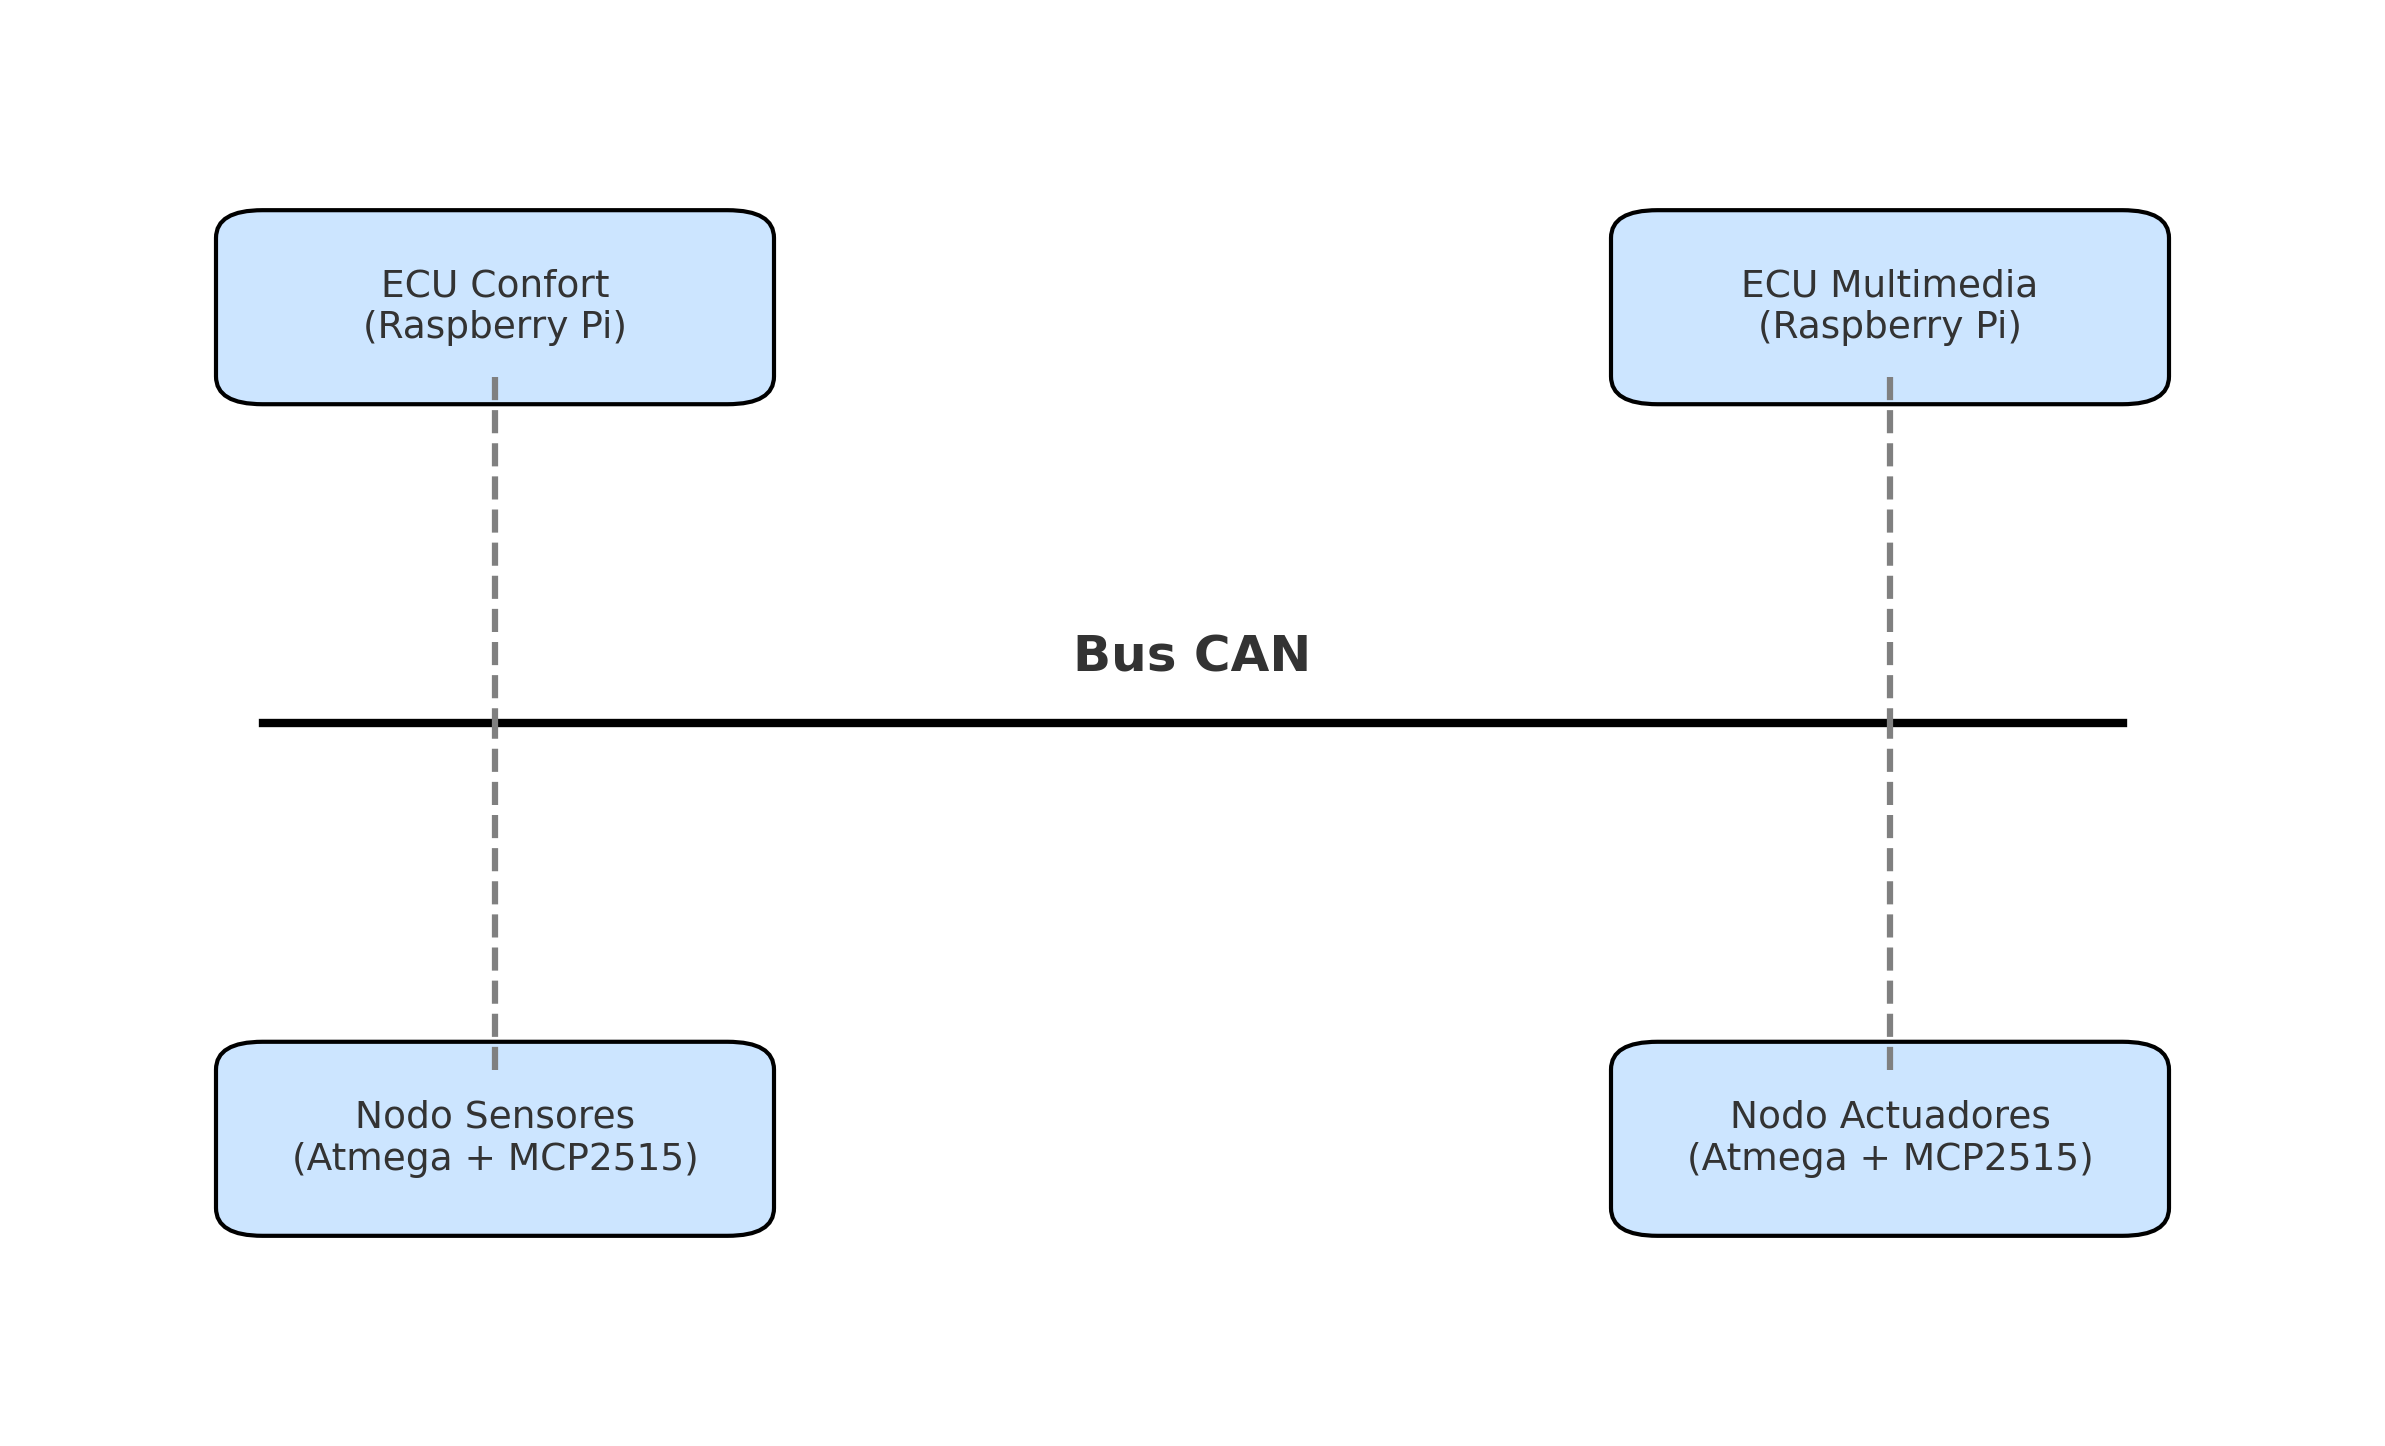
\includegraphics[width=0.9\textwidth]{figures/arquitectura_general.png}
    \caption{Arquitectura general del sistema de automatización distribuido.}
    \label{fig:arquitectura_general}
\end{figure}

\subsection{Diseño de hardware}

\subsubsection{Módulos de prueba}
Para la fase inicial de validación se emplearán módulos comerciales de \textbf{MCP2515} conectados a microcontroladores Atmega y Raspberry Pi. Esto permitirá probar la comunicación CAN sin necesidad de diseñar hardware propio.

\subsubsection{Placas personalizadas}
En la etapa final se diseñarán placas electrónicas que integren:
\begin{itemize}
    \item Controlador CAN MCP2515.
    \item Microcontrolador Atmega (para nodos simples).
    \item Interfaces de conexión a sensores (temperatura, humedad, presión).
    \item Actuadores (relés para ventanas, salidas digitales para iluminación).
\end{itemize}

\subsection{Diseño de software}

\subsubsection{ECUs (Raspberry Pi)}
Las ECUs estarán programadas en \textbf{Rust}, utilizando \texttt{Tauri} para las interfaces gráficas. Las funciones principales incluyen:
\begin{itemize}
    \item Procesamiento de mensajes CAN entrantes y salientes.
    \item Control de audio y multimedia.
    \item Interfaz gráfica para el usuario en pantalla integrada.
    \item Integración del módulo de control por voz local.
    \item Comunicación Bluetooth con la aplicación móvil.
\end{itemize}

\subsubsection{Nodos secundarios (Atmega)}
Cada nodo estará encargado de un conjunto específico de funciones, implementadas en \textbf{Rust embebido}, incluyendo:
\begin{itemize}
    \item Lectura de sensores (temperatura, humedad, presión).
    \item Control de actuadores mediante relés y salidas digitales.
    \item Comunicación CAN mediante MCP2515.
\end{itemize}

\subsubsection{Aplicación móvil}
La aplicación móvil se desarrollará en \textbf{React Native} con soporte inicial para Android. Sus funciones serán:
\begin{itemize}
    \item Conexión al vehículo vía Bluetooth.
    \item Monitoreo de datos en tiempo real (estado de ventanas, clima, sensores).
    \item Control remoto de funciones de confort y multimedia.
    \item Envío de comandos de voz hacia la ECU multimedia.
\end{itemize}

\subsection{Control por voz mediante inteligencia artificial}

El sistema integrará un motor de reconocimiento de voz local, con librerías como \textbf{Vosk} o \textbf{PocketSphinx}, que permitirá ejecutar comandos básicos sin conexión a internet. Entre las funciones iniciales se consideran:
\begin{itemize}
    \item Apertura y cierre de ventanas.
    \item Activación o desactivación del climatizador.
    \item Control de reproducción multimedia (play, pausa, siguiente).
    \item Consulta de datos de sensores (temperatura interior, humedad).
\end{itemize}

\subsection{Flujo de comunicación}

El flujo general de datos en el sistema es el siguiente:
\begin{enumerate}
    \item El usuario interactúa con la aplicación móvil o mediante comandos de voz.
    \item La ECU multimedia recibe la orden y la transmite por el bus CAN.
    \item El nodo correspondiente interpreta el mensaje y ejecuta la acción sobre el actuador o sensor.
    \item El estado actualizado se devuelve por el bus CAN y puede visualizarse en la app o en la interfaz de la ECU multimedia.
\end{enumerate}

Este flujo asegura una integración coherente y escalable de todas las funcionalidades, replicando en un vehículo antiguo las características de los sistemas modernos de automoción conectada.

\subsection{Desarrollo}
\subsubsection{Módulos de temperatura del habitáculo}

Para automatizar el climatizardor en un futuro, necesitamos poder conocer la temperatura, con cierta precisión, en
el interior del vehículo. Actualmente disponemos de varios sensores en el mercado que nos permiten medir la 
temperatura pero, todos disponen de un margen de error que se arrastra en cada lectura. Con el fin de reducir
el error del sensor, se plantea dividir el habitáculo del vehículo en 4 cuadrantes de forma que dispongamos
de un sensor por cada cuadrante.

\begin{figure}[H]
    \centering
    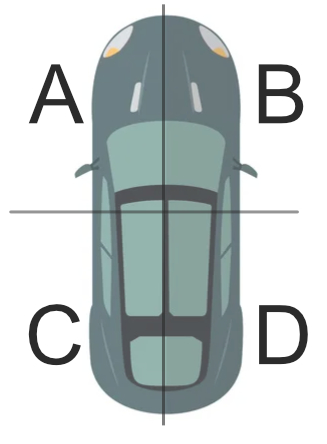
\includegraphics[width=4cm]{figures/clima-cuadran.jpg}
    \caption{Diagrama de los cuadrantes del vehículo.}
    \label{fig:climatización_cuadrantes}
\end{figure}

Mediante la división en cuadrantes tendremos a nuestra disposición 4 mediciones con las
que podremos realizar una media ponderada que será la medición más cercana a la realidad.\\

Esta media de mediciones se nos hace obligada, en parte, por la definición de temperatura, pues no es más que
la energía cinética de un sistema termodinámico, medición que sufre severas alteraciones debido a cualquier 
radiación directa de infrarojos.\textit{(Esto se puede observar si el sensor se deja al sol directo, la temperatura 
se disparará pero no será la temperatura del sistema termodinámico que es el habitáculo)}.

\subsubsection*{Componentes}

Para el desarrollo de los sensores de temperatura usaremos un sensor de grado médico para disponer de mayor precisión,
el \textbf{TMP117} en su empaquetado SMD. Este sensor nos permite una comunicación $I^2C$ y una precisión de 0,10 ºC,
lo que nos resulta atractivo para poder precisar la temperatura ambiente. \\

Como cerebro del sistema, durante las pruebas, se plantea usar un \textbf{Atmega 328P}, un microcontrolador de 8 
bits con soporte para reloj de hasta 16 MHz.

Para el producto final se plantea optimizar el diseño y reducir costes usando un \textbf{AtTiny87} que nos permite
usar tanto $I^2C$ como \textit{ISP} para la comunicación entre sensor y transreceptor CAN.


\subsubsection*{Diagrama del circuito}

\includepdf[pages={2}]{figures/TP-0010U001.pdf}
